\documentclass[9pt,compress,xcolor={table}]{beamer}

\usepackage{polyglossia}
\setmainlanguage{english}

\usetheme{hsrm}
\setbeameroption{show notes}

\usepackage{tabularx,ragged2e}
\usepackage{booktabs}
\usepackage{dtklogos}
\usepackage{tikz}
\usetikzlibrary{mindmap,backgrounds}
\usepackage{arydshln}
\usepackage{chngpage}
\usepackage{natbib}
\usepackage{multicol}
\usepackage[caption=false]{subfig}
%\usepackage[natbib=true, bibstyle=authoryear, citestyle=authoryear-comp, backend=bibtex]{biblatex}

\graphicspath{ {../../../resources/images/vectors/}{../../../resources/images/bits/} }

\title{Smart usage of context information for the analysis, design, and generation of power-aware policies for mobile sensing apps}

\subtitle{Phd research proposal}

\author{Rafael Pérez-Torres}

\institute{Center for Research and Advanced Studies of the National Polytechnic Institute\\LTI {\Medium Cinvestav}}

\date{\today}

\begin{document}

\maketitle

% Introduce elements
\section*{Structure}
\begin{frame}
  \frametitle{Structure}
  \tableofcontents[hideallsubsections]
\end{frame}


%!TEX root = ../slides.tex
\section{Introduction}
\subsection{Motivation}
\begin{frame}{Research background}{Motivation}
\begin{figure}[tb]
  \centering
  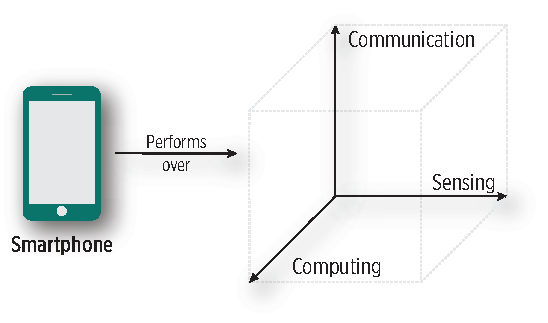
\includegraphics[width=0.4\textwidth]{vectors/smartphone-dimensions-v2}
  \caption{The advances in the communication, computing and sensing dimensions of mobile devices contribute to their acceptance by society~\cite{Islam2014}.}  
\end{figure}

\begin{block}{\small \textbf{Motivation}}
{
  \small
\begin{itemize}
  \item The sensing dimension enables \emph{context-awareness} in mobile devices, such as the smartphone.
  \item Battery advances are slower than those of other smartphone components~\cite{Kjaergaard2012}, growing 5-10\% yearly~\cite{Ma2012,Evarts2015}, a critical issue for the \textbf{mobile sensing applications}.
  % \item Battery advances are slower than those of other smartphone components~\cite{Kjaergaard2012}, growing 5-10\% yearly~\cite{Ma2012,Evarts2015}.
  % \item The energy constraint is critical for the continuous access to sensors required by \textbf{mobile sensing applications}. 
  \item Scientific efforts have been done for achieving the energy efficiency of the GPS location provider.
  \item The understanding of mobility could augment the location-awareness of the smartphone for many purposes, such as energy savings and the development of Mobility Based Services (MBSs).
  % \item As a high level of abstraction, mobility can be characterized as a sequence of frequently visited places (stay points).
\end{itemize}
}
\end{block}
\end{frame}

% \begin{frame}{Research background}{Motivation}
% \begin{block}{\small \textbf{Motivation}}
% {
%   \small
%    \begin{itemize}
%      \item For the sensing dimension, scientific efforts have been done for achieving the energy efficiency of the GPS location provider.
%      \item The understanding of mobility could augment the location-awareness of the smartphone for many purposes, such as energy savings and the development of Mobility Based Services (MBSs).
%      \item As a high level of abstraction, mobility can be characterized as a sequence of frequently visited places (a.k.a. stay points).
% \end{itemize}
% }
% \end{block}
% \end{frame}

\subsection{Research background}
%\subsection{Problem statement}
\begin{frame}{Research background}{Problem statement}
\small
\vspace{-0.5cm}
\begin{itemize}
  \item The understanding of mobility is possible at different spatial-temporal scales:
\end{itemize}

\begin{exampleblock}{\small \textbf{Fine-grain mobility patterns identification}}
 \begin{itemize}
    \item They refer to the transportation mode employed by user when moving between stay points.
    \item Given a set of values $\mathcal{V} = v_{acc~1},v_{acc~2},\ldots,v_{acc~n}$ obtained from accelerometer in the time interval $[t_1,t_2]$, identify fine-grain mobility information:
\begin{equation*}
  \text{\textbf{FineGrainMobilityIdentifier}}(\mathcal{V}) \rightarrow p_S \in \{ \text{static, walking, biking, vehicle} \}
\end{equation*}
with each $v_{acc~i} \in \mathcal{V}$ composed as $\langle acc_x,acc_y,acc_z,t \rangle$.
  \end{itemize} 
\end{exampleblock}

\begin{exampleblock}{\small \textbf{Coarse-grain mobility patterns identification}}
 \begin{itemize}
   \item They refer to motion at a large spatial scale related to user visiting stay points.
   \item \sloppy Given a set of values $\mathcal{V} = v_{gps~1},v_{gps~2},\ldots,v_{gps~n}$ obtained from GPS location provider in time interval $[t_1,t_2]$, identify coarse-grain mobility information:
\begin{equation*}
    \text{\textbf{CoarseGrainMobilityIdentifier}}(\mathcal{V}) \rightarrow p_S \in \{ \text{new stay point, arrival, departure} \}
\end{equation*}
with each $v_{gps~i} \in \mathcal{V}$ composed associated $\langle lat, lon, t \rangle$.
 \end{itemize}
\end{exampleblock}
\end{frame}


\begin{frame}{Research background}{Problem statement}
\small

\begin{exampleblock}{\small \textbf{Sensors sampling adaptation}}
\begin{itemize}
\item Given a set of coarse and fine-grain mobility patterns $\mathcal{P} = \{ p_{S_1}, p_{S_2}, \ldots, p_{S_n} \}$, and accuracy requirements of mobile app $req_{accuracy}$, implement a sampling policy for the adaptive duty cycling of sensors while reducing energy consumption:
\begin{equation*}
  \text{\textbf{PolicyGeneration}}( \mathcal{P}, req_{accuracy}) \longrightarrow{} \mathcal{S}_{conf}
\end{equation*}
where $\mathcal{S}_{conf} \rightarrow s, \mathcal{T}_{real}$ represents the sampling $\mathcal{T}_{real}$ that must be implemented for sensor $s$.
The $req_{accuracy}$ refers to the granularity of GPS sampling.
\end{itemize}
\end{exampleblock}

\begin{figure}[tb]
  \centering
  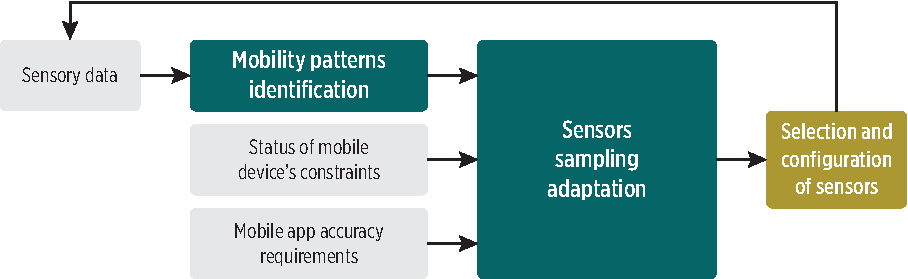
\includegraphics[width=0.7\textwidth]{vectors/problems-incorporation-v2}
  \caption{Interaction between problems.}
\end{figure}
\end{frame}

% \subsection{Hypothesis}
\begin{frame}{Research background}{Hypothesis}
\small
\begin{block}{\small \textbf{Hypothesis}}
\renewcommand{\baselinestretch}{1.4}
\begin{itemize}
  \item The energy consumption of continuous and extended location tracking could be reduced by means of a cognitive dynamic system that learns an expanded spatial-time model from mobility events detected from sensors data and that employs such model in a cognitive controller for dynamically adapting GPS sampling rate through sampling policies tailored to current mobility state.
\end{itemize}
\end{block}
\end{frame}


% \subsection{Objectives}
\begin{frame}{Research background}{Objectives}
\small
\begin{block}{\small \textbf{Main objective}}
\begin{itemize}
  \item To reduce the energy consumption of mobile sensing apps, which perform continuous sensor sampling, through self-adapting power-aware policies generated from context information obtained from sensors data.
\end{itemize}
\end{block}

\begin{block}{\small \textbf{Particular objectives}}
\begin{itemize}
  \item To detect mobility patterns from context information obtained from an inertial sensor (accelerometer) and location provider (GPS).
  \item To generate an accurate representation of detected patterns for summarizing user mobility.
  \item To dynamically adapt GPS sampling rate by means of a cognitive controller that employs the learned mobility representation and accuracy requirements for implementing power-aware sampling policies.
  \item To ease the development of mobile sensing applications that require user location tracking, i.e., LBSs and MBSs, isolating the complexity of sensors access and the associated efficient energy management.
\end{itemize}
\end{block}
\end{frame}



% \subsection{Methodology}
\begin{frame}{Research background}{Methodology}
\small
\begin{block}{\small \textbf{Methodology}}
\begin{enumerate}
  \item \textbf{Revision of state of the art power-aware sensing techniques.}
  \item \textbf{Formal definition and selection of mobility patterns to be identified.}
  \item \textbf{Research on algorithms for detecting mobility patterns.}
  \item \textbf{Design of the \emph{Mobility Events Detector}.}
  \item \textbf{Design of adaptive policies for energy efficient usage of sensors.}
  \item \textbf{Design of the Cognitive Controller.}
  \item \textbf{Development of a middleware involving the \emph{Mobility Events Detector} and the Cognitive Controller for the Android platform.}
  \item Experimentation in terms of spatial-time accuracy and energy efficiency.
\end{enumerate}
\end{block}
\end{frame}


\section{Problem statement}

\subsection{Preamble}

\begin{frame}{Problem description}
  \begin{block}{Current state of energy management}
    \begin{itemize}
      \item MSA access sensors in a continuous way over long periods of time.
      \item Sensors usage impacts directly on battery.
      \item Current smart devices' processors are designed to manage the heavy interaction with the user and the execution of mobile apps.
      \item A continuous sensor reading is out of their current objectives \citep{Priyantha2011}.
      % \item Current mobile platforms do not include mechanisms to perform periodical readings from sensors.
      \item API’s\footnote{API refers to Application Programming Interface.} by manufacturers only accomplish generic tasks like turning on – off sensors
    \end{itemize}
  \end{block}
\end{frame}

\begin{frame}{Problem description}
  \begin{block}{What do we need?}
    \begin{itemize}
      % \item API’s\footnote{API refers to Application Programming Interface.} by manufacturers only accomplish generic tasks like turning on – off sensors
      \item \textbf{High level information about user's context remains ignored}.
      \item A special framework to generate smart policies for continuous sensor access.
      \item This framework should consider:
        \begin{itemize}
          \item Mobile app requirements (e. g. the precision in the sensor data collection).
          \item Mobile device constraints (e. g. the current level of battery).
          \item Threshold values for performing a smart sensor usage (e. g. the lowest battery level for avoiding a permanent sensor usage).
        \end{itemize}
    \end{itemize}
  \end{block}
\end{frame}

\begin{frame}{Problem description}
  \begin{block}{A possible solution is}
    \begin{itemize}
      \item A policy is a high level concept that defines the usage sensors should observe to keep low energy consumption and fulfill mobile app requirements.

      \item The \emph{smartness} of policies is achieved by leveraging information about the user’s context obtained from sensors data.
      \begin{itemize}
        \item The user’s context can be recognized by employing a pattern identifier mechanism that is fed by raw data collected by sensors.

        \item The pattern becomes the descriptor of user’s context, and is the input for a policy generator mechanism that produces the policy to adapt the sensor usage, reduce the energy consumption and achieve mobile app objectives.
      \end{itemize}
      
    \end{itemize}
  \end{block}
\end{frame}


\subsection{Pattern identification}

\begin{frame}{Problem statement}
  \begin{exampleblock}{Pattern identification}
    Given a set $V = \left\{v_{1}, v_{2}, \dotsc, v_{n}\right\}$ of data values read from sensor $S$ in the time interval $T = \left\{t_{1}, t_{2}, \dotsc, t_{n}\right\}$, find the behavior pattern $Pattern_{S}$ that represents the activity of user.

    \begin{equation}
      PatternIdentifier( V ) \longrightarrow{} Pattern_{S} \in Patterns
    \end{equation}

    Where $Patterns$ is a set of patterns that represent an interesting state in the user activity.
  \end{exampleblock}
\end{frame}


\subsection{Policy generation}

\begin{frame}{Problem statement}
  \begin{exampleblock}{Policy generation}
    Given the pattern $Pattern_{S}$ detected in data from sensor $S$, parameters for assigning weight to energy $eh$ and precision $ph$, and physical constraints status $pc$ of a mobile device, find a policy to adapt the duty cycle of sensors.

    \begin{equation}
      PolicyGeneration( Pattern_{S}, eh, ph, pc ) \longrightarrow{} DutyCycle_{S}
    \end{equation}
  \end{exampleblock}
\end{frame}

\section{Hypothesis and objectives}


\subsection{Hypothesis}

\begin{frame}{Hypothesis}
  \begin{exampleblock}{Hypothesis}
    \begin{itemize}
      \item Smart policies generated through contextual information can be employed to reduce the energy consumption in a mobile device when performing continuous sensor readings.
    \end{itemize}    
  \end{exampleblock}
\end{frame}


\subsection{Objectives}

\begin{frame}{Objectives}
  \begingroup
    \setbeamercolor{block title}{bg=hsrmSec2Dark}
    \setbeamercolor{block body}{bg=hsrmSec2}
    
    \begin{block}{Main objective}
      \begin{itemize}
        \item Reduce energy consumption when performing continuous sensor readings in mobile devices by making use of context information.
      \end{itemize}
      
    \end{block}

    \begin{block}{Particular objectives}
      \begin{itemize}
        \item Identify behavior patterns which can provide meaningful context information from raw data collected by sensors.
        \item Generate smart policies for sensor usage from context information, mobile app requirements and mobile device constraints.
      \end{itemize}
    \end{block}
  \endgroup
\end{frame}

\section{State of art} 
\label{sec:state_of_art}
This section introduces a description and classification of works aiming to address the energy problem generated by employing sensors continuously in mobile sensing apps.
A special focus is given to the pure software techniques, which will be pursued during the development of this research.

\subsection{Approaches for addressing the energy issue}
\label{sub:approaches_for_addressing_the_energy_issue}

As stated, the advances produced in several technological fields have contributed to the acceptance of the smart devices, like the smartphone, by society \cite{Lane2010,Ra2012}.
However, although computing and storage capacity issues have been partially addressed and solved with every new generation of mobile devices, the energy consumption is still an open issue because of the slow rhythm in technological advances in batteries and because of the inclusion of newer and more sophisticated sensors that impose a higher energy demand.

In this sense, the battery consumption concern has been under research since the introduction of mobile devices into the market, and also shows an evolution in the objectives pursued by scientists. 

The research in energy management in mobile devices started with broad techniques and guidelines applied when building mobile application systems.
In \cite{Mayo2003} the authors address the energy consumption issue from a design point of view by introducing the idea of the \emph{requirements-aware energy scale-down} approach. 

This approach states that both hardware and software elements should scale their features and energy usage to meet a variety of design points.
According to it, if there are no hard energy constraints, the software can use the hardware components at maximum performance in order to accomplish the mobile app requirements.
On the other hand, in case of energy constraints the mobile app must be aware and react accordingly by modifying --- via software --- the hardware usage for consuming less energy and still accomplish the application requirements.
The described work was implemented targeting different hardware elements like screen, processor and wireless radio communication interfaces.
For example, the screen implementation aims the design of energy aware GUI's.
Such GUI's change the luminescence and color of non-active portions of the screen to reduce power consumption, as shown in the Figure \ref{fig-scaling-down-screen-usage}.

\begin{figure}
        \centering
        \begin{subfigure}[b]{0.3\textwidth}
                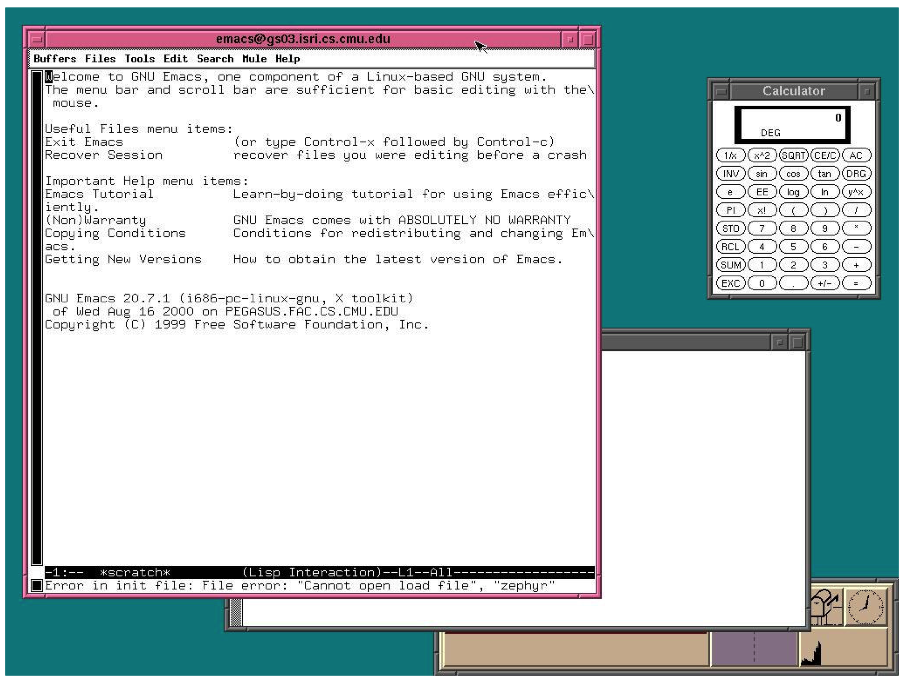
\includegraphics[width=\textwidth]{energy-aware-gui-1}
                \caption{Original interface}
                \label{fig:energy-aware-gui-1}
        \end{subfigure}
        ~
        \begin{subfigure}[b]{0.3\textwidth}
                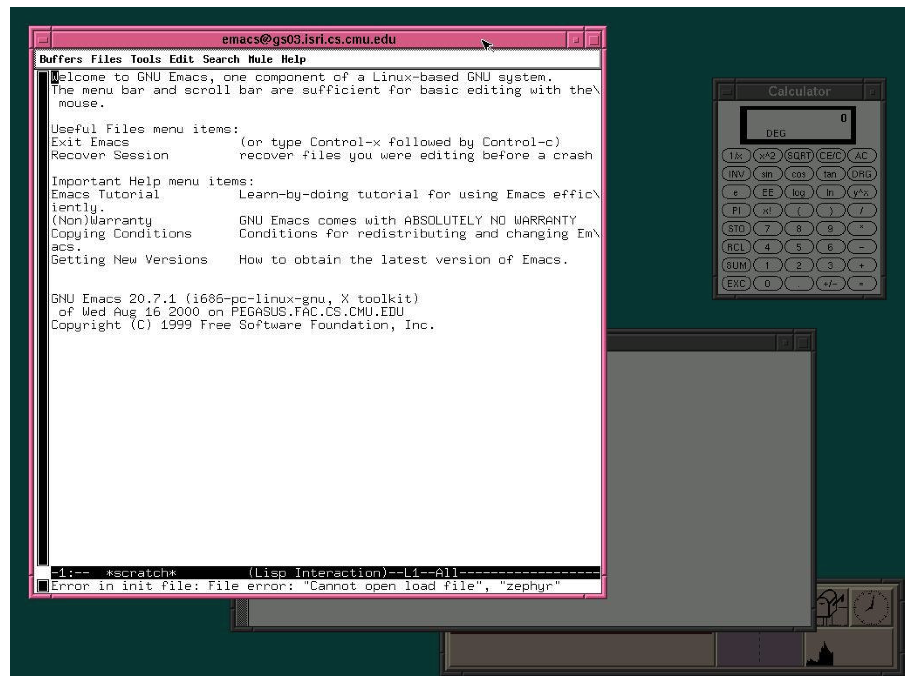
\includegraphics[width=\textwidth]{energy-aware-gui-2}
                \caption{Background half dim}
                \label{fig:energy-aware-gui-2}
        \end{subfigure}
        ~
        \begin{subfigure}[b]{0.3\textwidth}
                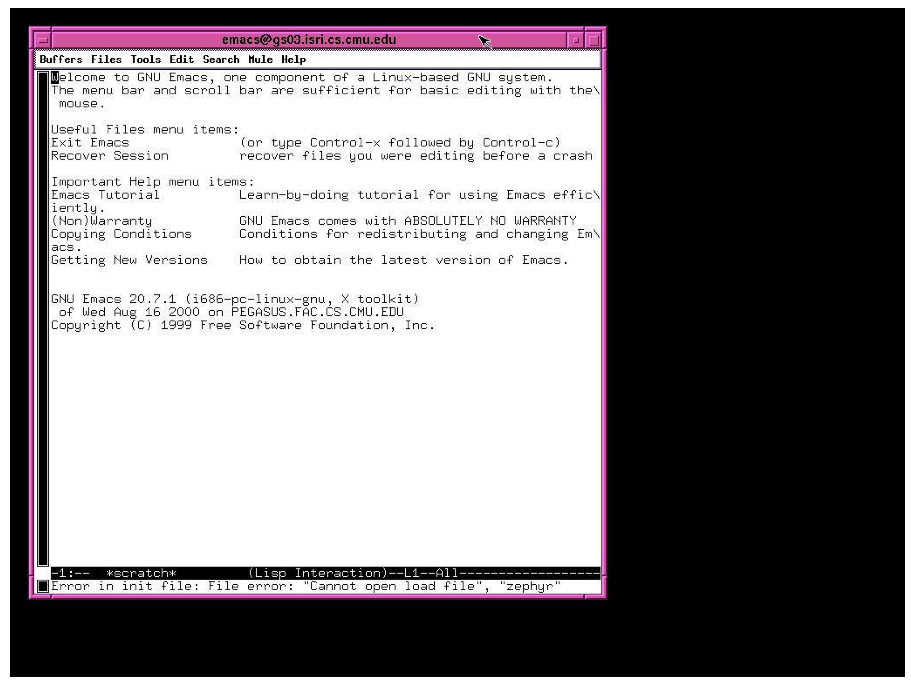
\includegraphics[width=\textwidth]{energy-aware-gui-3}
                \caption{Background fully dim}
                \label{fig:energy-aware-gui-3}
        \end{subfigure}
        \caption[An example of energy aware GUI by \protect\cite{Mayo2003}]{An example of energy aware GUI proposed by \protect\cite{Mayo2003}}
        \label{fig-scaling-down-screen-usage}
\end{figure}

The idea of \emph{requirements-aware energy scale-down} approach serves as a base for the creation of specific techniques for addressing the energy consumption issue.
However, the work introduced by authors focused on broad guidelines that, while helpful, left behind important details that can be obtained from contextual information of user.
It is noteworthy that at the time of the coinage of this approach the smart devices proliferation was in its infancy.

Currently, the popularity of smartphones and the mobile sensing apps have made the energy issue evident and specific mechanisms have been proposed to address it.
A revision of the literature shows that brooadly previous works can be categorized into are three families of techniques to face the energy issue (Figure \ref{fig:approaches-taxonomy}): 

\begin{itemize}
  \item Pure hardware.
  \item Hardware-software.
  \item Pure software.
\end{itemize}

The pure-hardware approach is located at hardware level and is agnostic of the entire software platform.
The hardware-software approach is located at the lowest levels of the mobile OS in connection with hardware elements.
It can be seen as the development of new hardware drivers.
Finally, the pure-software approach is located at top of the mobile OS stack and it is agnostic of the hardware platform.
Works under this approach make use of the API offered by the mobile OS for accessing sensors, collect data, analyze these data and readapt the usage of sensors.

\begin{figure}
\centering
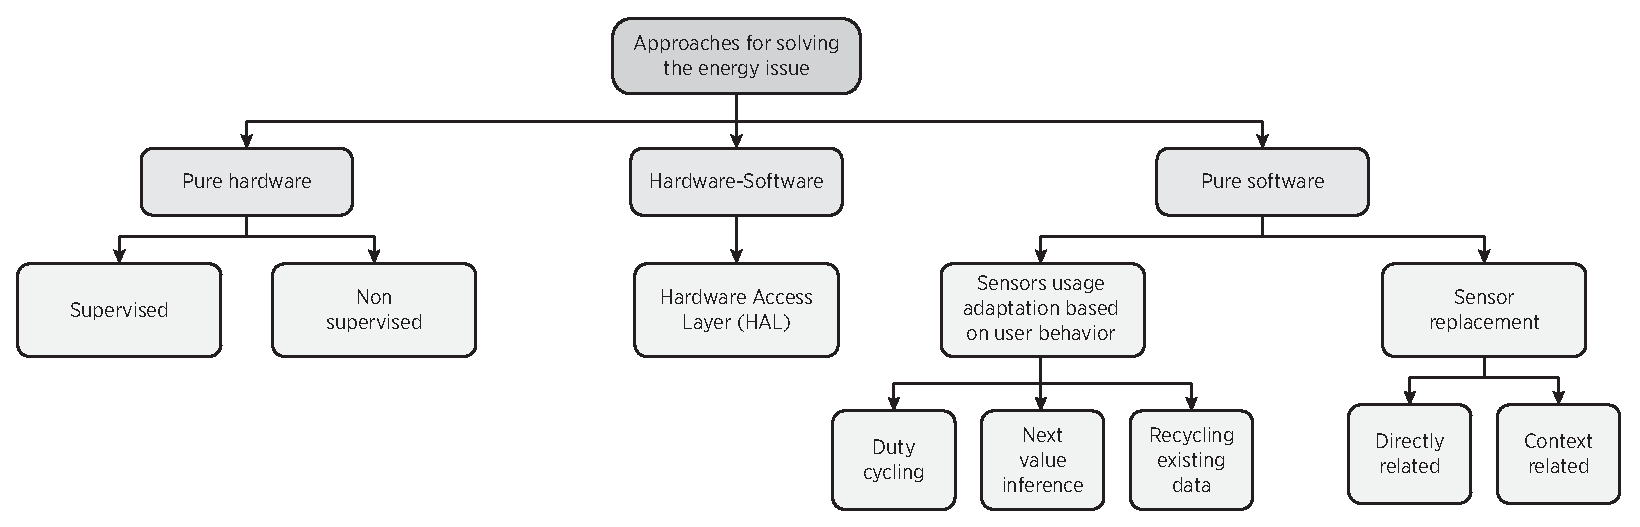
\includegraphics[width=\textwidth]{approaches-taxonomy}
\caption[Taxonomy of approaches for solving the energy issue]{Taxonomy of approaches for solving the energy issue.}
\label{fig:approaches-taxonomy}
\end{figure}

As can be seen in Figure \ref{fig:cross-layer-approaches}, the energy issue is a cross-layer problem that can be analyzed and addressed from several perspectives.
It is noteworthy that although there is a taxonomy of approaches, the solutions found in literature may include a combination of these techniques.
This is a suggestion of the complexity of the problem and even about the evolution of the techniques, since ideas proved to be working efficiently in software soon or later are implemented directly in hardware. 
\begin{figure}
\centering
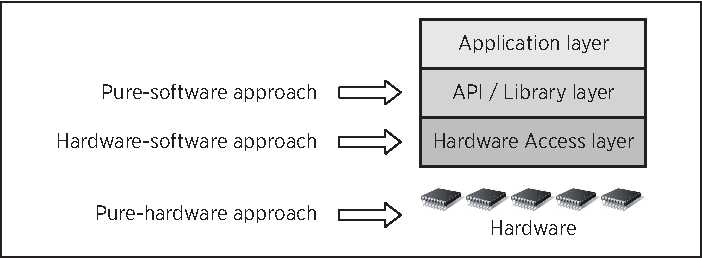
\includegraphics[scale=0.7]{cross-layer-approaches}
\caption[Energy issue as an OS cross-platform problem]{The relation between approaches for solving the energy issue and layers of a mobile platform.}
\label{fig:cross-layer-approaches}
\end{figure}

The Figure \ref{fig:approaches-description} shows the implementation of the three approaches seen from the perspective of the hardware platform.
It is interesting to note that the scope of the pure hardware approach is limited to the adaptation of the different physical variables introduced to the hardware components.
The adaptation of these variables, for example voltage and frequency illustrated in the figure, allows the definition of the power states of the different components, like the idle, active and other statuses.


The same Figure \ref{fig:approaches-description} also allows to detect the main purpose of the hardware – software approach, which is to define periods to keep sensors turned on or off, building a \emph{hardware access layer} above the bolts and nuts of the hardware platform.
Note in the Figure that the usage of the sensor is dictated by a square signal. When this signal has a high value, it turns the sensor on, whereas when it has a low value turns the sensor off. 
The generation of the square signal in this approach is typically done by lower layers of the mobile platform or even by a basic mobile app.


Finally, this Figure \ref{fig:approaches-description} shows the scope of the pure software approach.
Note that in this case, there is also a square signal involved in the behavior of the platform, but instead of controlling just a single sensor it is manipulating several of them.
The generation of this square signal is provided by the smartness present in the mobile app.
Only by leveraging context information it is possible to instruct this complex management of sensors.

% The Figure \ref{fig:approaches-description} shows how the different approaches are implemented in a hardware platform. Note that the pure hardware approach modifies directly the frequency and voltage introduced to the hardware circuits, defining the power states of the components.

% In the same figure, it can be seen that the hardware-software approach defines periods to keep the same sensor turned on or off, building a \emph{hardware access layer} above the bolts and nuts of the platform.

% Finally, the same figure shows that the pure software approach tries to define an even higher layer for modifying the behavior of the different sensors present in the mobile platform. The duty cycling of different sensors can be manipulated in order to obtain high level information --- meaningful for user --- and at the same time lowering the impact on battery.

The Table \ref{tbl:state-of-art-works} shows a set of works found in the literature that aim to solve the energy issue in mobile sensing apps.
An important aspect of these works is that due to their differences in approaches and purpose, it is not possible to perform a direct comparison of them \cite{Vallina-Rodriguez2013}.
The columns considered in the table refers to:
\begin{itemize}
  \item The authors and year of publication of the work.
  \item The approach followed by the work, including the specific variants implemented.
  \item The sensors employed in the work.
  \item The machine learning techniques employed in the work.
  \item The mobile platform where the work was implemented or simulated.
\end{itemize}
Such columns allow to identify the main characteristics present in these works.


{
\scriptsize
\begin{tabularx}{1.0\linewidth}%
  {
  >{\setlength{\hsize}{.6\hsize}\centering\arraybackslash}X
  >{\setlength{\hsize}{.6\hsize}\centering\arraybackslash}X
  >{\setlength{\hsize}{.5\hsize}\centering\arraybackslash}X
  >{\setlength{\hsize}{.8\hsize}\centering\arraybackslash}X
  >{\setlength{\hsize}{.6\hsize}\centering\arraybackslash}X
  }
  \caption{State of art works aiming to address the energy issue in MSA}\tabularnewline
  \toprule
  \textbf{Work} & \textbf{Approach} & \textbf{Sensors involved} & \textbf{Machine Learning Technique} & \textbf{Platform implementation}\tabularnewline
  \midrule
  \endfirsthead

  \toprule
  \textbf{Work} & \textbf{Approach} & \textbf{Sensors involved} & \textbf{Machine Learning Technique} & \textbf{Platform implementation}\tabularnewline
  \midrule
  \endhead

  \midrule
  \multicolumn{5}{c}{\emph{Continue in next page}}\tabularnewline
  \bottomrule
  \endfoot

  %\midrule
  %F1 & F2 & F3 & F4 & F5\\
  %\tabularnewline
  \bottomrule
  \tabularnewline
  \caption{State of art works aiming to address the energy issue in MSA \label{tbl:state-of-art-works}}
  \endlastfoot
  
  \cite{Constandache2009} &
      PS - Sensor usage based on behavior: NVI, DC &
      GPS, Wi-Fi interface, GSM network &
      Custom heuristic with Linear prediction &
      Data collection using Symbian on Nokia N95 phone. Experiments simulated.
      \tabularnewline
      \cmidrule(r){1-5}

      \cite{Kjaergaard2009} &
      PS - a) Sensor usage based on behavior: DC. \newline b) Sensor replacement: DR. &
      GPS, accelerometer &
      Dynamic programming &
      Symbian on Nokia N95 with Python scripts
      \tabularnewline
      \cmidrule(r){1-5}

      \cite{Zhuang2010} &
      HS - HAL &
      GPS, accelerometer &
      Simple decision rule &
      Android 1.5 on G1 Android Development Phone
      \tabularnewline
      \cmidrule(r){1-5}

      \cite{Perez2010} &
      PS - Sensor usage based on behavior: DC &
      GPS &
      Simple decision rule &
      Simulation
      \tabularnewline
      \cmidrule(r){1-5}

      \cite{Lin2010} &
      PS - a) Sensor usage based on behavior: DC, NVI. \newline b) Sensor replacement: DR. &
      GPS, Wi-Fi interface, Bluetooth, Cell tower data &
      Hidden Markov Models and a Bayesian estimation framework &
      Both emulation using datasets obtained from Microsoft and apps running on Android G1 smartphone.
      \tabularnewline
      \cmidrule(r){1-5}

      \cite{Lu2010} &
      PS - Sensor usage based on behavior: DC &
      Accelerometer, GPS, microphone &
      Decision Tree, Markov Decision Process and Gaussian Mixture Models &
      Nokia N95, Apple iPhone
      \tabularnewline
      \cmidrule(r){1-5}

      \cite{Priyantha2011} &
      PH - NA &
      Accelerometer, compass, gyroscope &
      None &
      Custom Hardware on unspecified smartphone phone
      \tabularnewline
      \cmidrule(r){1-5}

      \cite{Perez-Torres2012} &
      PS - Sensor usage based on behavior: DC &
      GPS &
      Simple decision rule &
      Android 2.3.3 on Samsung Galaxy S phone
      \tabularnewline
      \cmidrule(r){1-5}

      \cite{Srinivasan2012} &
      PS - Sensor usage based on behavior: DC &
      Accelerometer &
      Decision Tree &
      Tizen OS on Samsung Galaxy II phone and Android on Nexus S phone.
      \tabularnewline
      \cmidrule(r){1-5}

      \cite{Apple2015} &
      PH - A &
      Accelerometer, compass, gyroscope &
      Not available &
      iOS 8 in iPhone 5s or newer
      \tabularnewline
      \cmidrule(r){1-5}

      \cite{Zhang2013} &
      PS - a) Sensor usage based on behavior: DC. \newline b) Sensor replacement: DR &
      GPS, accelerometer &
      Gaussian Process Regression &
      Android 4.0 on Google Nexus S phone
      \tabularnewline
      \cmidrule(r){1-5}

      \cite{Chon2014} &
      PS - a) Sensor usage based on behavior: DC, NVI, RED. \newline b) Sensor replacement: CR &
      GPS, WiFi interface, Cell tower data &
      Hidden Markov Models &
      Android 2.2 phones.
      \tabularnewline
      \cmidrule(r){1-5}
      
      \cite{Yurur2014} &
      PS - Sensor usage based on behavior: NVI, DC &
      Accelerometer &
      Hidden Markov Models &
      Simulated in Matlab. Implemented on BlackBerry Storm II 9550 phone.
      \tabularnewline
      \cmidrule(r){1-5}

      \cite{Man2014} &
      PS - a) Sensor usage based on behavior: DC. \newline b) Sensor replacement: CR &
      GPS, accelerometer &
      Simple decision rule &
      Android 4.1.4 on Samsung Galaxy SIII i9300 phone
      \tabularnewline
      \cmidrule(r){1-5}

      \cite{Donohoo2014} &
      PS - a) Sensor usage based on behavior: DC. \newline b) Sensor replacement: DR &
      GPS, WiFi network, Cell tower data &
      Linear Discriminant Analysis, Linear Logistic Regression, Neural Network and K - Nearest Neighbor Several &
      Android 2.3.3 phones
      \tabularnewline

  \end{tabularx}
  }

In next sections a brief description of the pure hardware and hardware-software approaches is presented, followed by a detailed review of the pure software approach since the special features and advantages offered by it.
Inside each description some of the works presented in the Table \ref{tbl:state-of-art-works} are also reviewed.

\begin{figure}
\centering
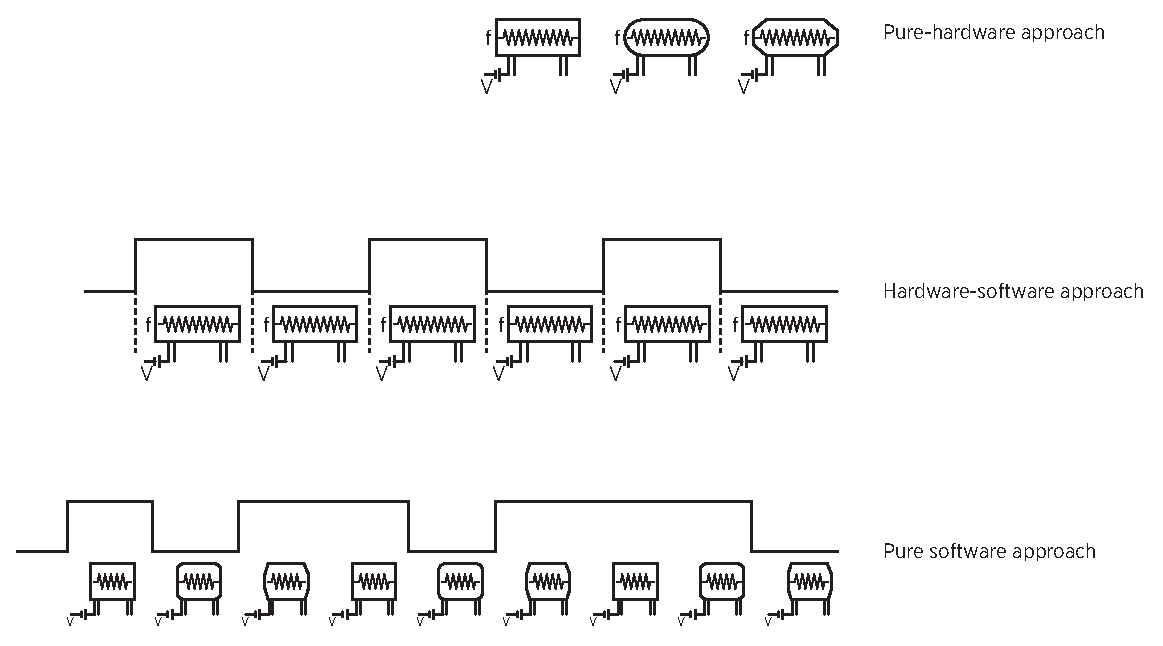
\includegraphics[scale=0.7]{approaches-description}
\caption[Approaches seen from hardware perspective]{The approaches seen from a hardware perspective.}
\label{fig:approaches-description}
\end{figure}

\subsubsection{Pure hardware approach}

Despite the fact current mobile processors include features at the electronic level like DPM\footnote{DPM, Dynamic Power Management} and DVFS\footnote{DVFS, Dynamic Voltage and Frequency Scaling} that are helpful to reduce the energy consumed by them, these techniques are not enough to solve the energy issue in mobile platforms.
The major drawback with the usage of these features is the complexity of the mobile processors, whose static power consumption remains high when the processor is not in sleep mode \cite{Priyantha2011}.
Additionally, the current architecture of most mobile platforms require that for the correct operation of the phone, other components have to be operational, which increases the energy consumption.

This approach is focused in adapting physical features of hardware components in order to reduce the energy consumption.
The most used physical features are the frequency and voltage introduced to the hardware elements.
In this way, the hardware designers define and introduce the different operational states of the physical components of the platform.

Works under this approach typically involve a hardware rearrangement to exploit the previously mentioned features.
This redesign implies the isolation of all of the components associated with the measurement of physical signals inside a new unit with a dedicated low power processor.
Such change must not carry a modification inside the mobile apps' logic.

This new hardware unit can obtain a substantial reduction in the energy consumption since it is energy aware by design.
The basic behavior involves that the sensors report their readings to the embedded low power processor, which is capable of doing light computing operations like filtering.
While the hardware unit is working on reading and filtering data, the rest of the smartphone's hardware platform is able to reach its sleep mode.

%The pure hardware approach can be materialized following two distinct implementations, based on the level of data complexity that the platform can handle.
Depending on the ability to process data and discover contextual information by itself, the pure hardware approach can be implemented in two different ways, namely, the not autonomous and the autonomous variants.

\subparagraph{Not autonomous variant}
\label{subp:not_autonomous_variant}

The \textbf{not autonomous} variant does not have knowledge about the information that is handled and it is restricted to receive sensor data requests and deliver data without running any sort of filtering or processing.

An example of the not autonomous variant is LittleRock \cite{Priyantha2011}.
Its design includes a special unit in charge of the access to sensors.
When any mobile app requires to perform sensing tasks it has the option to employ the LittleRock unit or use it only as a bridge and access directly to sensors.
The relevant features of this design are:

\begin{itemize}
  \item \textbf{Power independence:} LittleRock is powered directly from battery and not from other internal electronic items.
  Because of this, the main circuitry can be turned off when the phone is in sleep mode and keep LittleRock accessing to sensors.
  
  \item \textbf{Interrupt:} LittleRock offers interruption features, making it possible to wake up the phone and inform it about events discovered in data delivered by sensors.
  
  \item \textbf{Re-purposing:} LittleRock allows to reprogram its main processor to adapt the processing of sensor data and achieve mobile app requirements.
\end{itemize}

The experimentation conducted by authors indicates that LittleRock can operate up to 830 days when this and the phone are in sleep mode using a 1340 mAh battery.
Among the results, it is noteworthy that LittleRock is faster than the phone itself do collect a single sample of data from sensors due to the complexity of the software stack that the main processor has to handle.

Another relevant example of the supervised variant is reported in \cite{Choudhury2008}.
Despite the fact this work was not implemented in a smartphone unit, it also introduces a mobile sensing platform (MSP) that is composed in a similar way than LittleRock.
This MSP is basically a sensor board attached to a wireless node that includes a 32 bits ARM7 processor, Bluetooth interface and a compact flash bay for storage.
It can be noted that the MSP is representing the extra hardware unit with sensors and a dedicated low power processor, which can deliver the collected data via Bluetooth to an external computing unit for analysis and classification tasks.


\subparagraph{Autonomous variant}
\label{subp:autonomous_variant}

The \textbf{autonomous variant} is also able to deliver raw data, but additionally can detect higher level information thanks to the data processing algorithms.
For example, it might measure the distance covered by user, the amount of steps done, or identify the type of activity performed by the user (no movement, walking, running, etc.) completely by itself.


The autonomous variant has been already implemented in the Apple iPhone.
Starting from the iPhone 5s model, this smartphones family includes an ARM coprocessor that is in charge of interacting with several sensors like accelerometer, gyroscope and magnetometer in order to obtain data about user's fitness \cite{Sathiah2013}.

Apple has introduced a software API into the iPhone OS, the Core Motion Framework \cite{Apple2015}, that allows mobile app developers to make use of the new hardware architecture and to access and consume this information.
The Core Motion Framework is able to deliver information refering to amount of steps or distance that user has covered and even the type of activity performed by him.
Additionally, this API allows requests for raw data from sensors being the update frequency the only mandatory argument.

Despite the fact this implementation will lead to energy savings, it presents two major drawbacks.
The first one is that the step counter mechanism is always running in the background even if no applications are requesting data.
The second one is that this implementation does not provide support for continuous readings and lacks the idea of self adapting the sensor's duty cycle in order to reduce energy consumption.

A common problem of any hardware approach resides in that hardware designers can not foresee the needs of any future mobile development and implement them directly in the circuits.
In this sense, the effort of hardware designers is affected by a trade off between the features provided out-of-the box and the flexibility features offered by the produced hardware platform.

\subsubsection{Hardware-software approach}

Another approach found in literature describes a combination of hardware and software techniques to optimize the energy consumption in continuous sensing mobile apps.

This approach leverages physical information about sensors and basic data from context information in order to create basic rules to decide the best moment for turning sensors on and off.

% This technique aims to contribute with a reviewed and improved software API that allows to allocate computational and sensing tasks in components others than the predefined by the platform's original design.

By knowing the hardware platform, it is possible to change the behavior of the elements and employ them in a different manner.
An example of this idea is to enable an additional low power processor in the smartphone to execute any arbitrary instruction instead of the main processor.
Since the smartphone's processor can be kept idle there is a potential energy saving.

The work presented in \cite{Ra2012} leverages the presence of several low power processors (LP) in the latest smartphones.
The utilization of these LP's can be done by exposing their functionality through a layered API.

Through several simulations, authors show that such processors can bring substantial energy savings, specially when executing frequent sampling \& buffering and basic arithmetic operations.

That work describes two main challenges, the selection of a suitable LP and guidelines for deciding where to allocate the execution of a given task.
To select an adequate LP, the key factor is the wake up transition delay in terms of energy. So, any processor with a small wakeup transition delay is suitable as LP.
For deciding where to perform the execution of a task, the next guidelines are proposed:
\begin{itemize}
  \item \textbf{Execution in main processor:} {Tasks found to be more efficient in the main processor should be executed there, ignoring the transition penalty}.
  \item \textbf{Execution in LP:} {Tasks found to be more efficient in the LP, and that are very frequent within the mobile app, should be executed in the LP. Sampling and buffering tasks belong to this category}.
  \item \textbf{Execution in main or in LP:}{Tasks found to be more efficient in the LP, and  that are not frequent within the mobile app, should be executed in the LP. However, a special mechanism to evict them should be included. This might happen when tasks of other mobile apps request the LP}.
\end{itemize}


% \begin{table}
%   \centering
%     \scriptsize
%     \begin{tabularx}{1.0\linewidth}{>{\centering}X>{\centering}X>{\centering}X>{\centering}X>{\centering}X}
%       \toprule
%       \textbf{Work} & \centering{\textbf{Approach}} & \centering{\textbf{Sensors involved}} & \centering{\textbf{Machine Learning Technique}} & \centering{\textbf{Platform implementation}}
%       \tabularnewline
%       \midrule
      
%       \cite{Constandache2009} &
%       PS - Sensor usage based on behavior: NVI, DC &
%       GPS, Wi-Fi interface, GSM network &
%       Custom heuristic with Linear prediction &
%       Data collection using Symbian on Nokia N95 phone. Experiments simulated.
%       \tabularnewline
%       \cmidrule(r){1-5}

%       \cite{Kjaergaard2009} &
%       PS - a) Sensor usage based on behavior: DC. \\b) Sensor replacement: DR. &
%       GPS, accelerometer &
%       Dynamic programming &
%       Symbian on Nokia N95 with Python scripts
%       \tabularnewline
%       \cmidrule(r){1-5}

%       \cite{Zhuang2010} &
%       HS - HAL &
%       GPS, accelerometer &
%       Simple decision rule &
%       Android 1.5 on G1 Android Development Phone
%       \tabularnewline
%       \cmidrule(r){1-5}

%       \cite{Perez2010} &
%       PS - Sensor usage based on behavior: DC &
%       GPS &
%       Simple decision rule &
%       Simulation
%       \tabularnewline
%       \cmidrule(r){1-5}

%       \cite{Lin2010} &
%       PS - a) Sensor usage based on behavior: DC, NVI. \\b) Sensor replacement: DR. &
%       GPS, Wi-Fi interface, Bluetooth, Cell tower data &
%       Hidden Markov Models and a Bayesian estimation framework &
%       Both emulation using datasets obtained from Microsoft and apps running on Android G1 smartphone.
%       \tabularnewline
%       \cmidrule(r){1-5}

%       \cite{Lu2010} &
%       PS - Sensor usage based on behavior: DC &
%       Accelerometer, GPS, microphone &
%       Decision Tree, Markov Decision Process and Gaussian Mixture Models &
%       Nokia N95, Apple iPhone
%       \tabularnewline
%       \cmidrule(r){1-5}

%       \cite{Priyantha2011} &
%       PH - NA &
%       Accelerometer, compass, gyroscope &
%       None &
%       Custom Hardware on unspecified smartphone phone
%       \tabularnewline
%       \cmidrule(r){1-5}

%       \cite{Perez-Torres2012} &
%       PS - Sensor usage based on behavior: DC &
%       GPS &
%       Simple decision rule &
%       Android 2.3.3 on Samsung Galaxy S phone
%       \tabularnewline
%       \cmidrule(r){1-5}

%       \cite{Srinivasan2012} &
%       PS - Sensor usage based on behavior: DC &
%       Acceleromete &
%       Decision Tree &
%       Tizen OS on Samsung Galaxy II phone and Android on Nexus S phone.
%       \tabularnewline
%       \cmidrule(r){1-5}

%       \cite{Apple2013} &
%       PH - A &
%       Accelerometer, compass, gyroscope &
%       Not available &
%       iOS 8 in iPhone 5s or newer
%       \tabularnewline
%       \cmidrule(r){1-5}

%       \cite{Zhang2013} &
%       PS - a) Sensor usage based on behavior: DC.\\b) Sensor replacement: DR &
%       GPS, accelerometer &
%       Gaussian Process Regression &
%       Android 4.0 on Google Nexus S phone
%       \tabularnewline
%       \cmidrule(r){1-5}

%       \cite{Chon2014} &
%       PS - a) Sensor usage based on behavior: DC, NVI, RED.\\b) Sensor replacement: CR &
%       GPS, WiFi interface, Cell tower data &
%       Hidden Markov Models &
%       Android 2.2
%       \tabularnewline
%       \cmidrule(r){1-5}
      
%       \cite{Yurur2014} &
%       PS - Sensor usage based on behavior: NVI, DC &
%       Accelerometer &
%       Hidden Markov Models &
%       Simulated in Matlab. Implemented on BlackBerry Storm II 9550 phone.
%       \tabularnewline
%       \cmidrule(r){1-5}

%       \cite{Man2014} &
%       PS - a) Sensor usage based on behavior: DC.\\b) Sensor replacement: CR &
%       GPS, accelerometer &
%       Simple decision rule &
%       Android 4.1.4 on Samsung Galaxy SIII i9300 phone
%       \tabularnewline
%       \cmidrule(r){1-5}

%       \cite{Donohoo2014} &
%       PS - a) Sensor usage based on behavior: DC.\\b) Sensor replacement: DR &
%       GPS, WiFi network, Cell tower data &
%       Linear Discriminant Analysis, Linear Logistic Regression, Neural Network and K - Nearest Neighbor Several &
%       Android 2.3.3 phones
%       \tabularnewline

%       \bottomrule
%     \end{tabularx}
%     \caption{State of art works aiming to address the energy issue in MSA}
%     \label{tbl:state-of-art-works}
% \end{table}


\section{Methodology}
\subsection{Methodology}
\begin{frame}{Methodology}
  \small
  \setbeamertemplate{enumerate item}{\Roman{enumi}}
  \begin{block}{Steps}
    \begin{enumerate}%[label=\bfseries Step \Roman*]
      %\renewcommand{\labelenumii}{Task \arabic{enumii}:}
      \item \textbf{Research on the characteristics of data delivered by sensors, in this case the GPS receiver.}

        % It can bring theoretical fundaments to improve the representation of data, for example achieving data compression.
        Identify special characteristics of GPS data that may trigger the study of techniques like outliers elimination, noise reduction, filtering, windowing, and framing to launch pre-processing of data delivered by sensors.

        % \begin{enumerate}
        %   \item Research on characteristics of data delivered by GPS receiver.
        % \end{enumerate}

      \item \label{itm:def-sel-mob-pttrns} \textbf{Definition and selection of mobility patterns to be identified.}

        This step is needed to identify the target mobility patterns that will be employed later in the pattern identifier element.

        % Examples of these mobility patterns are static, walking, running, vehicle at high speed, etc.

        The set of target mobility patterns defined here will be part of the input for the pattern identifier element.

        % \begin{enumerate}
        %   \setcounter{enumii}{1}
        %   \item Coding a sample app to gather GPS data from the smartphone.
        %   This app will access GPS receiver in a continuous and permanent way.
        %   \item Analysis of data delivered by the mobile app.
        %   \item Selection of the mobility patterns that will be recognized by the platform.
        %   \item Creation of the formal definition of mobility pattern.
        % \end{enumerate}
    \end{enumerate}
  \end{block}
\end{frame}

\begin{frame}{Methodology}
  \small
  \setbeamertemplate{enumerate item}{\Roman{enumi}}
  \begin{block}{Steps}
    \begin{enumerate}
      \setcounter{enumi}{2}
      \item \label{itm:research-alg-pttrn-rec} \textbf{Research and adaptation of algorithms to detect mobility patterns of user based on data delivered by GPS.}

        % Once the characteristics of data collected by sensors have been studied and the patterns to be identified have been defined, it is needed to detect a mobility pattern from these data.
        
        The pattern is helpful to get information about user's context and therefore in the generation of policies.
        
        The selected algorithms should consider the constraints present in mobile devices.

        % \begin{enumerate}
        %   \setcounter{enumii}{5}
        %   \item Research on algorithms for pattern recognition from GPS data.
        %   \item Definition of metrics for evaluating algorithms.
        %   \item Evaluation of algorithms.
        %   \item Selection of proper algorithm(s), discussing the best conditions for its (their) usage.
        % \end{enumerate}

      \item \textbf{Creation of the pattern identifier element (PIE).}

        This element must identify the pattern from data collected by sensors by employing the algorithm(s) selected in the Step \ref{itm:research-alg-pttrn-rec}.
        
        The pattern identified must be included in the set of mobility patterns defined in the Step \ref{itm:def-sel-mob-pttrns}.

        % \begin{enumerate}
        %   \setcounter{enumii}{9}
        %   \item Definition of parameters accepted by the PIE and their formal representation.
        %   \item Elaboration of the PIE.
        %   % \item Fine tunning of the PIE towards its usage in a constrained device (the smartphone)
        % \end{enumerate}

    \end{enumerate}
  \end{block}
\end{frame}

\begin{frame}{Methodology}
  \small
  \setbeamertemplate{enumerate item}{\Roman{enumi}}
  \begin{block}{Steps}
    \begin{enumerate}
      \setcounter{enumi}{4}

      \item \textbf{Creation of the policy generator element (PGE).}

        It includes the definition of a formal representation of policies.
        
        This policy generator element will obtain the duty cycle that the GPS receiver must implement to perform the next GPS reading.

        % \begin{enumerate}
        %   \setcounter{enumii}{11}
        %   \item Definition of parameters accepted by the PGE and their representation.
        %   \item Creation of the formal definition of \emph{policy}.
        %   \item Elaboration of the PGE.
        %   % \item Fine tunning of the PGE towards its usage in a constrained device (the smartphone)
        % \end{enumerate}

      \item \textbf{Development of a software element (SE) that integrates both PIE and PGE.}

        This software element will be implemented in the Android platform.
        
        % The Android platform is selected in this research because of its popularity, well documented SDK, and because its availability in the research center.

        % \begin{enumerate}
        %   \setcounter{enumii}{14}
        %   % \item Analysis and definition of logical elements involved in software abstractions.
        %   \item Definition of SE architecture.
        %   \item Research on Android API for specialized components related to sensor access and task-process management.
        %   \item Coding of the SE.
        % \end{enumerate}

      \item \textbf{Experimentation.}

        Key aspects are precision and energy saving.
        
        % Precision refers to the fidelity that data collected by employing policies maintain in relation to actual ground truth data.
        % This can be measured by executing data analysis processes over data collected by sensors through policies versus data collected without employing policies.
        
        % Energy saving refers to the reduction in the energy consumption that is obtained when applying policies versus the inter-built facilities of mobile operating systems.
        
        This step involves the definition of experiments and the development of mobile applications that employs the constructed software element.

        % \begin{enumerate}
        %   \setcounter{enumii}{17}
        %   \item Definition of experiments targeting energy saving and user tracking precision metrics.
        %   \item Development of mobile apps employing the SE for running the experimentation.
        %   \item Execution of the experimentation.
        %   \item Results analysis.
        % \end{enumerate}

    \end{enumerate}
  \end{block}
\end{frame}


\begin{frame}{Methodology}
  \begin{block}{Workflow of methodology}
    \begin{figure}
      \centering
      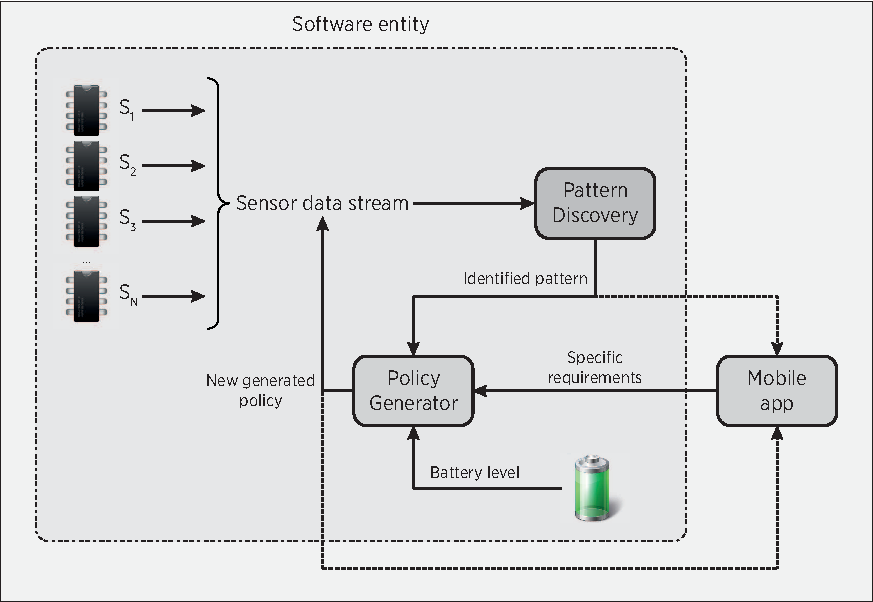
\includegraphics[scale=0.45]{methodology-stages}
      \caption[Methodology workflow]{Workflow described by the proposed methodology}
      \label{fig-methodology-workflow}
    \end{figure}
  \end{block}
\end{frame}

\section{Contributions}

\subsection{Contributions}

\begin{frame}{Contributions}
  \begin{block}{Contributions}
    \begin{itemize}
      \item A mechanism for detecting patterns (contextual information) from the data read by sensors of mobile devices (specifically the GPS receiver).
      \item A mechanism for generating policies for accessing sensors that considers mobile app requirements and information about user's context.
      \item A software element able to read data from sensors using the policies generated by the described mechanisms and transmit these data to an external server.
    \end{itemize}
  \end{block}
\end{frame}


\section{Schedule}

\subsection{Schedule}

\begin{frame}{Schedule}
  \definecolor{colorA}{gray}{0.85}
  \definecolor{colorB}{gray}{0.95}
  \definecolor{colorStep}{gray}{1}

  \newlength{\longitudCelda}
  \setlength{\longitudCelda}{75mm}

  \begin{table}[!h]
  {
    \scalebox{0.6}{
    \small
      \begin{tabular*}{16.5cm}{lp{\longitudCelda}*{12}{c}}
          & & \multicolumn{3}{ c: }{\tiny SEP '14 - AUG '15}  & \multicolumn{3}{ c: }{\tiny SEP '15 - AUG '16} & \multicolumn{3}{ c: }{\tiny SEP '16 - AUG '17} & \multicolumn{3}{ c }{\tiny SEP '17 - AUG '18} \\
          \cline{3-14}

          \multicolumn{2}{c:}{}
          & \tiny 1\textsuperscript{st} & \tiny 2\textsuperscript{nd} & \multicolumn{1}{c:}{ \tiny 3\textsuperscript{rd}}
          & \tiny 1\textsuperscript{st} & \tiny 2\textsuperscript{nd} & \multicolumn{1}{c:}{ \tiny 3\textsuperscript{rd}}
          & \tiny 1\textsuperscript{st} & \tiny 2\textsuperscript{nd} & \multicolumn{1}{c:}{ \tiny 3\textsuperscript{rd}}
          & \tiny 1\textsuperscript{st} & \tiny 2\textsuperscript{nd} &  \tiny 3\textsuperscript{rd} \\
          \cline{3-14}

          \rowcolor{colorStep}
          & \multicolumn{1}{c}{\scriptsize \textsc{Step I}}  & & & & & & & & & & & & \\
          % First year
          \rowcolor{colorA}
          1 & \multicolumn{1}{p{\longitudCelda}:}{Research on characteristics of data delivered by GPS receiver} &
          \cellcolor[gray]{0.3} & & &
          & & &
          & & &
          & & \\

          %\hdashline
          \rowcolor{colorStep}
          & \multicolumn{1}{c}{\scriptsize \textsc{Step II}}  & & & & & & & & & & & & \\

          \rowcolor{colorB}
          2 & \multicolumn{1}{p{\longitudCelda}:}{Coding a sample app to gather GPS data from smartphone} &
          \cellcolor[gray]{0.3} & & &
          & & &
          & & &
          & & \\

          \rowcolor{colorA}
          3 & \multicolumn{1}{p{\longitudCelda}:}{Analysis of data delivered by the mobile app} &
          \cellcolor[gray]{0.3} & & &
          & & &
          & & &
          & & \\

          \rowcolor{colorB}
          4 & \multicolumn{1}{p{\longitudCelda}:}{Selection of the mobility patterns} &
          \cellcolor[gray]{0.3} & \cellcolor[gray]{0.3} & &
          & & &
          & & &
          & & \\

          \rowcolor{colorA}
          5 & \multicolumn{1}{p{\longitudCelda}:}{Creation of the formal definition of mobility pattern} &
          & \cellcolor[gray]{0.3} & &
          & & &
          & & &
          & & \\

          %\hdashline
          \rowcolor{colorStep}
          & \multicolumn{1}{c}{\scriptsize \textsc{Step III}}  & & & & & & & & & & & & \\

          \rowcolor{colorB}
          6 & \multicolumn{1}{p{\longitudCelda}:}{Research on algorithms for pattern recognition from GPS data} &
          & \cellcolor[gray]{0.3} & &
          & & &
          & & &
          & & \\

          \rowcolor{colorA}
          7 & \multicolumn{1}{p{\longitudCelda}:}{Definition of metrics for evaluating algorithms} &
          & \cellcolor[gray]{0.3} & \cellcolor[gray]{0.3} &
          & & &
          & & &
          & & \\

          \rowcolor{colorB}
          8 & \multicolumn{1}{p{\longitudCelda}:}{Evaluation of algorithms} &
          & & \cellcolor[gray]{0.3} &
          & & &
          & & &
          & & \\

          \rowcolor{colorA}
          9 & \multicolumn{1}{p{\longitudCelda}:}{Selection of proper algorithm(s)} &
          & & \cellcolor[gray]{0.3} &
          & & &
          & & &
          & & \\

          % Second year
          \rowcolor{colorStep}
          & \multicolumn{1}{c}{\scriptsize \textsc{Step IV}}  & & & & & & & & & & & & \\

          \rowcolor{colorB}
          10 & \multicolumn{1}{p{\longitudCelda}:}{Definition \& representation of parameters accepted by PIE} &
          & & &
          \cellcolor[gray]{0.3} & & &
          & & &
          & & \\

          \rowcolor{colorA}
          11 & \multicolumn{1}{p{\longitudCelda}:}{Elaboration of the PIE} &
          & & &
          \cellcolor[gray]{0.3} & \cellcolor[gray]{0.3} & &
          & & &
          & & \\

          %\hdashline
          \rowcolor{colorStep}
          & \multicolumn{1}{c}{\scriptsize \textsc{Step V}}  & & & & & & & & & & & & \\

          \rowcolor{colorB}
          12 & \multicolumn{1}{p{\longitudCelda}:}{Definition \& representation of parameters accepted by PGE} &
          & & &
          & & \cellcolor[gray]{0.3} &
          & & &
          & & \\

          \rowcolor{colorA}
          13 & \multicolumn{1}{p{\longitudCelda}:}{Creation of the formal definition of policy} &
          & & &
          & & \cellcolor[gray]{0.3} &
          & & &
          & & \\

          \rowcolor{colorB}
          14 & \multicolumn{1}{p{\longitudCelda}:}{Elaboration of the PGE} &
          & & &
          & & \cellcolor[gray]{0.3} &
          \cellcolor[gray]{0.3} & \cellcolor[gray]{0.3} & &
          & & \\

          %\hdashline
          \rowcolor{colorStep}
          & \multicolumn{1}{c}{\scriptsize \textsc{Step VI}}  & & & & & & & & & & & & \\

          \rowcolor{colorA}
          15 & \multicolumn{1}{p{\longitudCelda}:}{Analysis of elements involved into software abstractions} &
          & & &
          & & &
          & \cellcolor[gray]{0.3} & &
          & & \\

          \rowcolor{colorB}
          16 & \multicolumn{1}{p{\longitudCelda}:}{Research on Android API for specialized} &
          & & &
          & & &
          & \cellcolor[gray]{0.3} & &
          & & \\

          \rowcolor{colorA}
          17 & \multicolumn{1}{p{\longitudCelda}:}{Coding-development of the SE} &
          & & &
          & & &
          & \cellcolor[gray]{0.3} & \cellcolor[gray]{0.3} &
          & & \\

          %\hdashline
          \rowcolor{colorStep}
          & \multicolumn{1}{c}{\scriptsize \textsc{Step VII}}  & & & & & & & & & & & & \\

          % Fourth year
          \rowcolor{colorB}
          18 & \multicolumn{1}{p{\longitudCelda}:}{Definition of experiments} &
          & & &
          & & &
          & & \cellcolor[gray]{0.3} &
          & & \\

          \rowcolor{colorA}
          19 & \multicolumn{1}{p{\longitudCelda}:}{Development of mobile apps for running the experimentation} &
          & & &
          & & &
          & & \cellcolor[gray]{0.3} &
          & & \\

          \rowcolor{colorB}
          20 & \multicolumn{1}{p{\longitudCelda}:}{Execution of the experimentation} &
          & & &
          & & &
          & & \cellcolor[gray]{0.3} &
          \cellcolor[gray]{0.3} & & \\

          \rowcolor{colorA}
          21 & \multicolumn{1}{p{\longitudCelda}:}{Results analysis} &
          & & &
          & & &
          & & &
          \cellcolor[gray]{0.3} & & \\

          % Required tasks
          %\hdashline
          \rowcolor{colorStep}
          & \multicolumn{1}{c}{\scriptsize \textsc{Required tasks}}  & & & & & & & & & & & & \\

          \rowcolor{colorB}
          22 & \multicolumn{1}{p{\longitudCelda}:}{Related subject courses} &
          \cellcolor[gray]{0.3} & \cellcolor[gray]{0.3} & \cellcolor[gray]{0.3} &
          & & &
          & & &
          & & \\

          \rowcolor{colorA}
          23 & \multicolumn{1}{p{\longitudCelda}:}{Publication of results} &
          & & &
          & & &
          & & &
          \cellcolor[gray]{0.3} & \cellcolor[gray]{0.3} & \cellcolor[gray]{0.3} \\

          \rowcolor{colorB}
          24 & \multicolumn{1}{p{\longitudCelda}:}{Thesis writing} &
          & & &
          & & &
          & & &
          \cellcolor[gray]{0.3} & \cellcolor[gray]{0.3} & \cellcolor[gray]{0.3} \\

      \end{tabular*}
    }
  } % begin table
  \caption{Schedule of activities (each column represents a four months period)}
  \label{tbl-schedule}
  \end{table}
\end{frame}


% \section{References}

\bibliographystyle{unsrtnat}

%\begin{frame}{References}
\frame[allowframebreaks]{ 
		\bibliography{../../../resources/references/bibliography}  
}
% \end{frame}

\end{document}
